\section{Public Key Encryption}

Note: all codes in this section include a common header file, \texttt{Part1/p2\_common.h}, which can be found in Appendix \ref{code:2_common}.

%%%%%%%%%%%%%%%%%%%%%%%%%%%%%%%%%%%%%%%%%%%%%%%%%%%%%%%%%%%%%%%%%%%%%%%%%%%%%%%%
% \subsection{Background}
\setcounter{subsection}{1}

%%%%%%%%%%%%%%%%%%%%%%%%%%%%%%%%%%%%%%%%%%%%%%%%%%%%%%%%%%%%%%%%%%%%%%%%%%%%%%%%
\subsection{BIGNUM APIs}

For the following sections, I used these API.\footnote{This part of introduction referred to OpenSSL online documents: \url{https://www.openssl.org/docs/man1.1.1/man3}}

Function \texttt{BN\_new} is used to allocate and initialize a new \texttt{BIGNUM}.
Function \texttt{BN\_free} is used to free the components of the \texttt{BIGNUM}, and if it was created by \texttt{BN\_new()}, also the structure itself.
Function \texttt{BN\_dup} creates a new \texttt{BIGNUM} containing the value \texttt{from}.
\begin{verbatim}
  BIGNUM *BN_new(void);
  void BN_free(BIGNUM *a);
  BIGNUM *BN_dup(const BIGNUM *from);
\end{verbatim}

Function \texttt{BN\_bn2hex} is used to serialize a \texttt{BIGNUM} into a hex string.
Function \texttt{BN\_hex2bn} is used to deserialize a hex string into a \texttt{BIGNUM}.
\begin{verbatim}
  char *BN_bn2hex(const BIGNUM *a);
  int BN_hex2bn(BIGNUM **a, 
                const char *str);
\end{verbatim}

Function \texttt{BN\_sub\_word} subtracts a \texttt{BIGNUM} by \texttt{w}.
Function \texttt{BN\_mul} multiplies two \texttt{BIGNUM}s.
Function \texttt{BN\_mod\_inverse} calculates $a^{-1} \mod{n}$ and return a pointer to the result.
These three functions are used when calculating the private exponent $d$.

Function \texttt{BN\_mod\_exp} calculates modulus exponent. It is used when encrypting, decypting, signing and verifying.
\begin{verbatim}
  int BN_sub_word(BIGNUM *a, BN_ULONG w);
  int BN_mul(BIGNUM *r, BIGNUM *a, 
             BIGNUM *b, BN_CTX *ctx);
  BIGNUM *BN_mod_inverse(BIGNUM *r, 
                         BIGNUM *a, 
                         const BIGNUM *n,
                         BN_CTX *ctx);
  int BN_mod_exp(BIGNUM *r, BIGNUM *a, 
                 const BIGNUM *p,
                 const BIGNUM *m, 
                 BN_CTX *ctx);
\end{verbatim}

Some of the above functions requires a \texttt{BN\_CTX}, which is used to storage temporary \texttt{BIGNUM} and to cut down the overhead for allocating and releasing memory.
Function \texttt{BN\_CTX\_new} is used to allocate and initialize a \texttt{BN\_CTX} structure.
Function \texttt{BN\_CTX\_free} frees the components of the \texttt{BN\_CTX} and the structure itself.
\begin{verbatim}
  BN_CTX *BN_CTX_new(void);
  void BN_CTX_free(BN_CTX *c);
\end{verbatim}

For easier use of the functions, some helper functions are written in \texttt{p2\_common.h}, which can be found in Appendix \ref{code:2_common}.

%%%%%%%%%%%%%%%%%%%%%%%%%%%%%%%%%%%%%%%%%%%%%%%%%%%%%%%%%%%%%%%%%%%%%%%%%%%%%%%%
\subsection{Deriving the Private Key}

The algorithm to derive private exponent $d$ is stated as Algorithm \ref{alg:rsa_pqe_d}.
Command and output is screenshot as Fig.\ref{fig:p2_3}.
Code can be found in Appendix \ref{code:2_3}

\begin{figure}[b!]
\centering
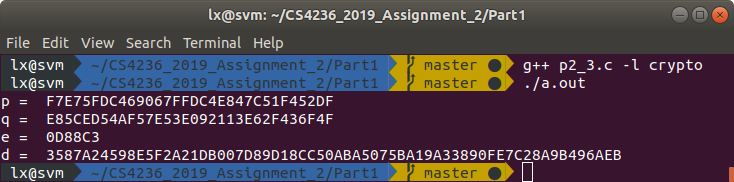
\includegraphics[width=\columnwidth]{pictures/p2_3.png}
\caption{
    Calculate private key exponent $d$
}
\label{fig:p2_3}
\end{figure}

\begin{algorithm}
\caption{Calculate private key exponent $d$}
\label{alg:rsa_pqe_d}
\begin{algorithmic}
\STATE \textbf{Input:} Private primes $p$,$q$ and public exponent $e$
\STATE \textbf{Output:} Private exponent $d$

\STATE $ n \gets pq $
\STATE $ \phi(n) \gets (p-1)(q-1) $
\STATE $ d \gets e^{-1} \mod{\phi(n)} $
\RETURN $ d $
\end{algorithmic}
\end{algorithm}

%%%%%%%%%%%%%%%%%%%%%%%%%%%%%%%%%%%%%%%%%%%%%%%%%%%%%%%%%%%%%%%%%%%%%%%%%%%%%%%%
\subsection{Encrypting a Message}

The algorithm to encrypt a message $m$ using RSA algorithm with public key $(n, e) $ is stated as Algorithm \ref{alg:rsa_enc}.
Command and output is screenshot as Fig.\ref{fig:p2_4}.
Code can be found in Appendix \ref{code:2_4}

\begin{algorithm}
\caption{RSA encrypt}
\label{alg:rsa_enc}
\begin{algorithmic}
\STATE \textbf{Input:} RSA public key $(n, e)$ and message $m$
\STATE \textbf{Output:} Ciphertext $c$

\STATE $ c \gets m^e \mod{n} $
\RETURN $ c $
\end{algorithmic}
\end{algorithm}

\begin{figure}[b!]
\centering
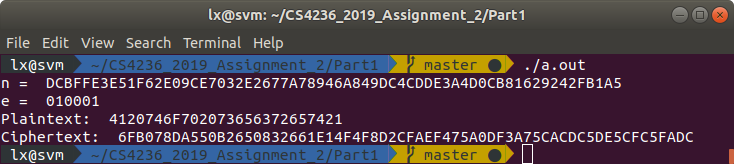
\includegraphics[width=\columnwidth]{pictures/p2_4.png}
\caption{
    RSA encrypt
}
\label{fig:p2_4}
\end{figure}

%%%%%%%%%%%%%%%%%%%%%%%%%%%%%%%%%%%%%%%%%%%%%%%%%%%%%%%%%%%%%%%%%%%%%%%%%%%%%%%%
\subsection{Decrypting a Message}

The algorithm to decrypt a ciphertext $c$ using RSA algorithm with private key $(n, d) $ is stated as Algorithm \ref{alg:rsa_dec}.
Command and output is screenshot as Fig.\ref{fig:p2_5}.
Code can be found in Appendix \ref{code:2_5}

\begin{algorithm}
\caption{RSA decrypt}
\label{alg:rsa_dec}
\begin{algorithmic}
\STATE \textbf{Input:} RSA private key $(n, d)$ and ciphertext $c$
\STATE \textbf{Output:} Plaintext $m$

\STATE $ m \gets c^d \mod{n} $
\RETURN $ m $
\end{algorithmic}
\end{algorithm}

\begin{figure}[!t]
\centering
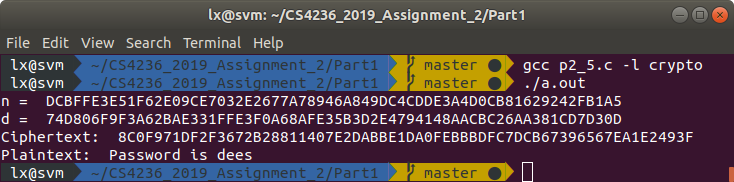
\includegraphics[width=\columnwidth]{pictures/p2_5.png}
\caption{
    RSA decrypt
}
\label{fig:p2_5}
\end{figure}

%%%%%%%%%%%%%%%%%%%%%%%%%%%%%%%%%%%%%%%%%%%%%%%%%%%%%%%%%%%%%%%%%%%%%%%%%%%%%%%%
\subsection{Signing a Message}
\label{subs:sign}

The algorithm to sign a message $m$ using RSA algorithm is completely the same as RSA decryption (Algorithm \ref{alg:rsa_dec}) which utilize the private key except that the output is called a signature.
Command and output is screenshot as Fig.\ref{fig:p2_6}.
Code can be found in Appendix \ref{code:2_6}

Note that when I changed \texttt{\$2000} to \texttt{\$3000}, the signature becomes different. Concretely, we changed 1 bit in the message. Then there are 123 different bits (in the total 256 bits) in the two signatures, which is nearly 50\% of all bits.

\begin{figure}[!t]
\centering
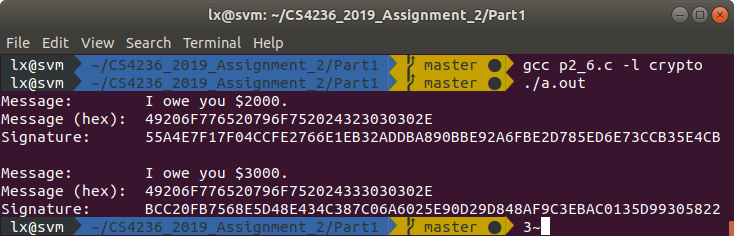
\includegraphics[width=\columnwidth]{pictures/p2_6.png}
\caption{
    RSA sign
}
\label{fig:p2_6}
\end{figure}

%%%%%%%%%%%%%%%%%%%%%%%%%%%%%%%%%%%%%%%%%%%%%%%%%%%%%%%%%%%%%%%%%%%%%%%%%%%%%%%%
\subsection{Verifying a Signature}

The algorithm to verify a signature using RSA algorithm is stated as Algorithm \ref{alg:rsa_verify}).
Command and output is screenshot as Fig.\ref{fig:p2_7}.
Code can be found in Appendix \ref{code:2_7}

From this example, it can be seen that 1 bit different in the two signature caused the recovered measurements completely different. They even don't have the same length.

This example and the one in Question \ref{subs:sign} show that there's a great diffusion property in RSA.

\begin{algorithm}
\caption{RSA verify}
\label{alg:rsa_verify}
\begin{algorithmic}
\STATE \textbf{Input:} RSA public key $(n, e)$, message $m$ and signature $S$
\STATE \textbf{Output:} \texttt{SUCCESS} or \texttt{FAIL}

\STATE $ s \gets m^e \mod{n} $

\IF {$S = s$} 
    \RETURN \texttt{SUCCESS}
\ELSE
    \RETURN \texttt{FAIL}
\ENDIF 

\end{algorithmic}
\end{algorithm}

\begin{figure}[!t]
\centering
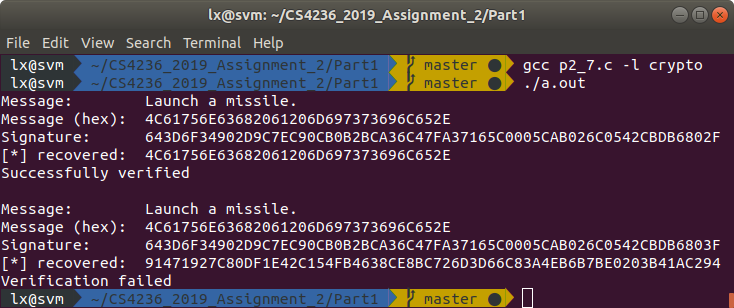
\includegraphics[width=\columnwidth]{pictures/p2_7.png}
\caption{
    RSA verify
}
\label{fig:p2_7}
\end{figure}